\documentclass{article}
\usepackage{graphicx}
\usepackage{tikz}
\usetikzlibrary{calc,trees,positioning,arrows,chains,shapes.geometric,%
    decorations.pathreplacing,decorations.pathmorphing,shapes,%
    matrix,shapes.symbols}

\begin{document}

Since the defocused images of seed particles are fuzzy rings, the task of
tracking the micron-scale particles is to identify the rings of various sizes
on each frame and reconstruct their trajectories. For this project, We have
developed a fast algorithm based on Hough Transform for particle tracking.
With the help of UFO parallel computing framework, we implement our new algorithm on
heterogeneous computing platforms with graphic cards. 


The old Matlab software uses template matching method based on order statistic
filter algorithm. However template matching is not efficient in dealing with
patterns of large sizes. Indeed it shows poor performance in searching for
rings with radius that is about 20 and larger pixels. In addition, when the
algorithm is implemented on parallel computing devices like GPUs, it can not
support patterns with arbitrary large radius, since the patterns can be too
large to be hold in device caches. Therefore we investigate on a new algorithm
based on Hough Transform (HT). We find that Hough Transform for circular
patterns can be efficiently carried out with Fast Fourier Transform. Our
approach is therefore both computing time and memory efficient.

The flow of our algorithm is shown in Fig. \ref{fig:alguptv}.  We first apply
standard image processing filters, such as local contrast enhancement and noise
reduction, to the input images. Then they are sent to HT filter. In our
problem, the standard procedure of edge detection before HT does not apply,
since the rings are fuzzy and do not have crisp edges. Our approach is to apply
HT filters without edge detection and devise an efficient blob detection
algorithm, because the HT votes tend to form blurred blobs at position of ring
centers.  In this step, most unwanted pixels are filtered out, leaving the rest
pixels as candidates for ring centers.  We further use a azimuthal filter to
eliminate the false positives in the candidates. The azimuthal filter is a test
on the pixel histogram in radius direction respect to the center of candidate
ring. The histogram calculated from true ring center shall show strong peak at
the position of ring radii. To identify the peaks, we have to apply a fitting
procedure with a Gaussian fitting function. The benefit is that the precisions
of ring centers and ring radius can be determined to pixel level. However,
the task is not suitable to be paralleled on GPUs.

The UFO framework let us develop software in OpenCL with relative ease and
distribute the more computational intensive part on to graphic cards. The UFO
framework also supports to stream images on to multiple GPUs on same or
different hosts.  It is our future work to speed up the software with a GPU
cluster. At the moment, we have use UFO to develop our software with GPU
acceleration.  Benchmarking on our particle tracking software shows that it
takes roughly 300 to process each frame on a computer with a Nvidia GTX Titan
GPU card and Xeon E3-1200 CPU.  


\tikzset{
>=stealth',
  punktchain/.style={
    rectangle, 
    rounded corners, 
    % fill=black!10,
    draw=black, very thick,
    text width=10em, 
    minimum height=3em, 
    inner sep=0.7em,
    text centered, 
    on chain},
  line/.style={draw, thick, <-},
  element/.style={
    tape,
    top color=white,
    bottom color=blue!50!black!60!,
    minimum width=8em,
    draw=blue!40!black!90, very thick,
    text width=10em, 
    minimum height=3.5em, 
    text centered, 
    on chain},
  every join/.style={->, thick,shorten >=1pt},
  decoration={brace},
  tuborg/.style={decorate},
  tubnode/.style={midway, right=2pt},
}

\begin{figure}
\centering
\begin{tikzpicture}
    [thick,scale=1.0,
      node distance=1.8em,
      every node/.style={scale=1.0},
      start chain=going below,]
     \node[punktchain, join] (intro) {Input image stream};
     \node[punktchain, join] (preprocessing) {
             Pre-processing:\\
             \emph{\footnotesize contrast adjustment,\\[-0.6em]
                                             denoising} };
     \node[punktchain, join] (hough)      {Hough Transform};
     \node[punktchain, join] (blob) {Hessian blob detection};
     \node[punktchain, join] (azimuth) {Post processing:\\
                                        \emph {\footnotesize Azimuthal filter} };
     \node[punktchain, join] (output) {Output stream};

          %Now, let us add some braches. 
  %% No. 1
  %\draw[tuborg] let
    %\p1=(risiko.west), \p2=(finans.east) in
    %($(\x1,\y1+2.5em)$) -- ($(\x2,\y2+2.5em)$) node[above, midway]  {Teori};
  %% No. 2
  %\draw[tuborg, decoration={brace}] let \p1=(disk.north), \p2=(makro.south) in
    %($(2, \y1)$) -- ($(2, \y2)$) node[tubnode] {Analyse};
  %% No. 3
  %\draw[tuborg, decoration={brace}] let \p1=(perfekt.north), \p2=(emperi.south) in
    %($(2, \y1)$) -- ($(2, \y2)$) node[tubnode] {Problemfelt};
\end{tikzpicture}
\caption{uptv algorithm}
\label{fig:alguptv}
\end{figure}


\begin{table}[t]
\centering
\begin{tabular}{c c}
\hline
\textbf{Algorithm} & \textbf{Benchmark} \\
\hline
Order Statistic Filter & 200~s \\
Hough Transform & 300~ms \\
\hline
\end{tabular}
\caption{Benchmark: Hough transform compared to order statistic filter algorithm.}
\end{table}

\begin{figure} 
    \centering 
    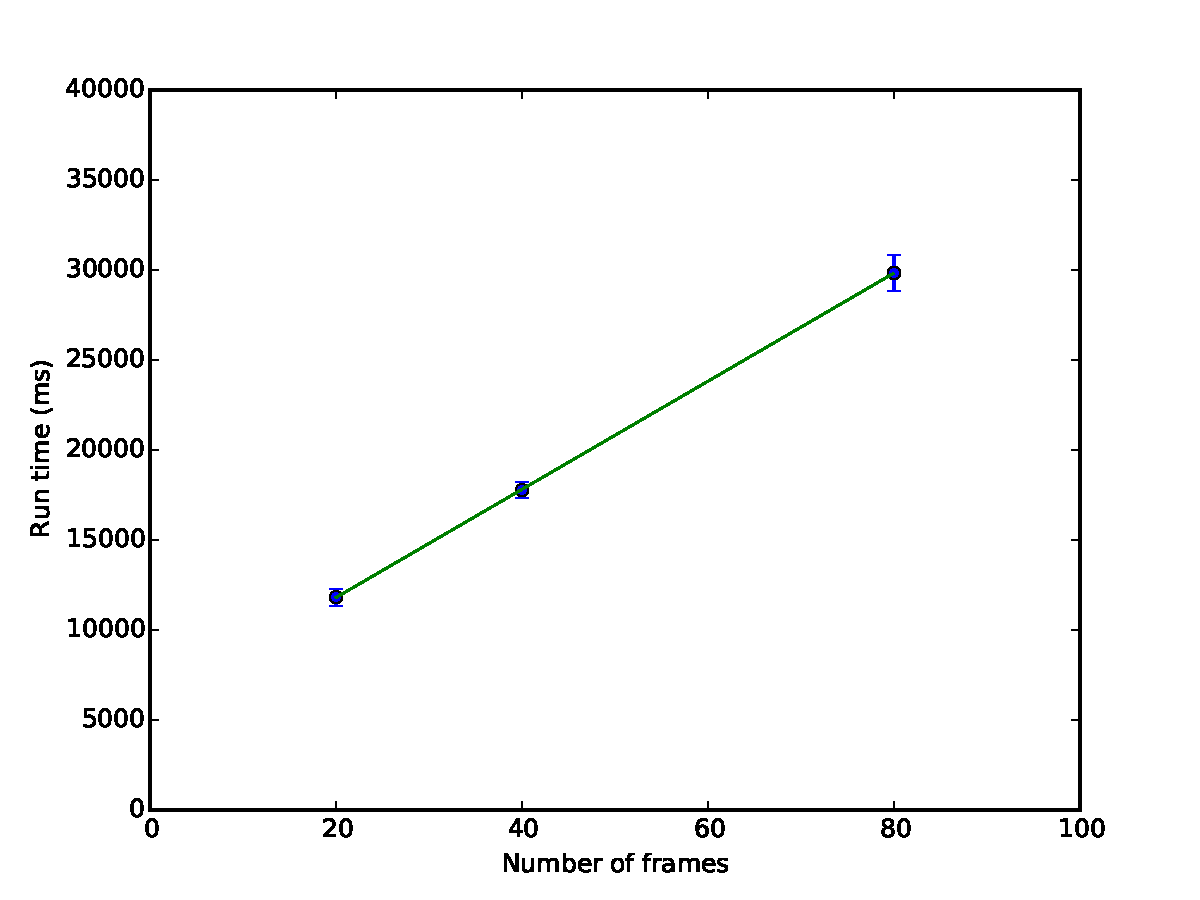
\includegraphics[width=0.8\textwidth]{fig_bc}
\caption{Performance measured with various number of frames. Fitting of the
data shows that the processing of image stream takes roughly 300 ms per frame
without initial setup time.} 
\end{figure}


\end{document}
